%%%%%%%%%%%%%%%%%%%%%%%%%%%%%%%%%%%%%%%%%%%%%%%%%%%%%%%%%%%%%%%%%%%%%%%%%%%%%%
% CONTRIBUTION TO THE MESONH BOOK1: "Bogusing for cyclones"
% Author: Olivier Nuissier, david Barbary
% Original : March 27, 2008
% Modification : February 16, 2009
%%%%%%%%%%%%%%%%%%%%%%%%%%%%%%%%%%%%%%%%%%%%%%%%%%%%%%%%%%%%%%%%%%%%%%%%%%%%%%%

\chapter{Bogusing for Cyclones}

\minitoc
\section{Introduction}
Mature tropical cyclones are very intense atmospheric disturbances with 
typical horizontal extent of several hundred to a thousand kilometers, 
occurring over the most earth's tropical oceanic regions. Wind, storm surges 
and inland flooding generally associated with tropical cyclones cause, 
every year, losing of human lives and major material damages in many 
countries of the tropical belt. Dedicated airborne missions performed over 
the Atlantic using Doppler radars, but also generally coastal Doppler 
measurements can permit to deduce kinematic and thermodynamic structure of 
the vortex. 

Meanwhile, since early of 70's, tropical cyclone modeling significantly 
improved with using of sophisticated parameterization schemes of convection, 
microphysics, turbulence, surface fluxes,... However, one major drawback of many 
numerical studies of tropical cyclone is the fact that the initial vortex, 
usually obtained from global analyses, is often ill-defined, too weak, and 
sometimes misplaced, leading to subsequent simulation of storm track, structure, 
and intensity.

The following approach is the one proposed by Nuissier et al. (2005) is which 
airborne Doppler radar data are used to define a 'specified vortex' for Meso-NH
model initialization.

\section{Method}


\subsection{Removal of the analyzed vortex}

To incorporate a hurricane-like vortex with realistic size, depth, and intensity 
in the Meso-NH initial conditions, it is first necessary to remove the weak 
vortex analyzed by global models. For this purpose, the scheme proposed by 
Kurihara et al. (1993 (hereafter KBR93), 1995) is applied.
It consists of using appropriate numerical  filters to extract the vortex
from the large-scale analysis and adding a vortex specified from observations.
This can be written symbolically as:

\begin{equation}
[h_{i}]=[h]-[h_{av}]+[h_{s}]
\label{hi}
\end{equation}

where $[h_{i}]$ is the initial field (that means zonal and meridian wind, thermal field and optionally the pressure field), $[h]$ is the global analysis, $[h_{av}]$ is 
the analyzed vortex and $[h_{s}]$ is the specified vortex. 

A low-pass filter with an exponential weighting function, following Barnes (1964),
 is first applied to the modified large-scale analysis field [h] over the outermost Meso-NH domain to 
remove features with wavelengths smaller than about 1200 km, the characteristic 
dimension of the analyzed vortex. The filtering radius is defined precisely by the condition $R_{filt}=\min(R_{Filt}^{User}; 1.25\times R_{Filt}^{Calculated})$ where $R_{Filt}^{User}$ is the maximal filtering radius giving by the user and $R_{Filt}^{Calculated}$ the calculated filtering radius following the condition ($[V_{T}<6\,\mbox{m.s}^{-1}$ and $ \partial V_{T} / {\partial r} <4.10^{-6}\,\mbox{s}^{-1}]$ or $V_{T}<3\,\mbox{m.s}^{-1}$), where $V_{T}$ is the tangential wind.
Using the same terminology as KBR93, this 
produces the basic field $[h_{b}]$, which is subtracted from $[h]$ to obtain the 
total disturbance field $[h_{d}]$:

\begin{equation}
[h]-[h_{b}]=[h_{d}]=[h_{av}]+[h_{nh}]
\label{hb}
\end{equation}

where $[h_{nh}]$ is the none-hurricane disturbance.

The next step consists of extracting $[h_{av}]$ from $[h_{d}]$. This is done 
using the same cylindrical filter as that proposed by KBR93:

\begin{equation}
h_{av}(r,\theta)=h_{d}(r,\theta)-[h_{d}(r_{0},\theta)E(r)+h_{d}(r_{0})(1-E(r))]
\end{equation}

where r and $\theta$ are the radius and the azimuth relative to the center  of the 
analyzed vortex, $r_{0}$ is the radius at which the value of weighting function 
E(r)=1, and $h_{d}(r_{0}$) is the mean value of $h_{d}(r,\theta$) for $r=r_{0}$ 
and $0\le\theta<2\pi$. The function E(r) (see Eq. (3.8) and Fig. 2b in 
KBR93) is an empirically determined exponential equation which increases smoothly 
from 0 at $r=0$ to 1 at $r=r_{0}$, with a smooth transition between the inner (i.e. 
hurricane component for $r<r_{0}$) and the outer regions (i.e. non-hurricane 
component for $r>r_{0}$).

\subsection{A 'specified vortex' derived from airborne Doppler radar observations}

After the analyzed vortex has been removed, the resulting environmental fields are 
used as new large-scale conditions, and interpolated over the other innermost Meso-NH 
domains. A symmetrical radar-derived vortex deduced from Doppler radar observations 
is then added to this modified large-scale field in every Meso-NH domains. This 
method is referred to as the 'Radar Vortex Conditioning' (RVC).

The wave number-0 component (symmetrical part) of the tangential wind is first 
deduced from the Extended Velocity-Track Display (EVTD) or Ground-Based 
Velocity-Track Display (GB-VTD) analysis (Roux and Marks 1996, Roux et al. 2004). Although the EVTD-derived velocities bring valuable information on the storm dynamic structure, they do not cover a large enough domain to properly define the specified vortex. Hence, an analytic model is used to describe the radial and vertical 
distribution of the tangential wind over a larger domain. The analytic wind 
$V_{T}(r,z)$, where $z$ is altitude, is defined through the 
formulation proposed by Holland (1980), as:

\begin{equation}
V_{T}(r,z)=\sqrt{ V_{Tmax}^2(z) \times \frac {\exp\left\lbrace 1- 1 / [r / RMW(z) ]^{B(z)} \right\rbrace }
{[r/RMW(z)]^{B(z)}} + \left[\frac{fr}{2}\right]^2 } - \left|\frac{fr}{2}\right|
\label{VT(r,z)}
\end{equation}

where $V_{Tmax}(z)$ is the maximum wind, $f$ is the Coriolis parameter, $RMW(z)$ is the radius of maximum wind, and $B(z)$ is a scaling parameter for the radial variation of the wind. We can notice that the tangential wind is not an axisymmetric field because of the Coriolis parameter. In order to avoid 
spurious variations of $V_{Tmax}$, $RMW$ and $B$ between the different levels, they 
suppose to obey the following relations with respect to z:

\begin{eqnarray}
\label{VTmax(z)}
V_{Tmax}(z) &=& V_{Tmax}(z=0) \left[1-\frac{z}{z_{max}} \right]^c\\
\label{RMW(z)}
RMW(z) &=& RMW_{0}\times \left[1 +\rho_{z}\times \frac{z}{z_{max}}+\rho_{zz}\times \left[\frac{z}{z_{max}} \right]^2\right]\\
\label{B(z)}
B(z) &=& B_{0}\times\left[1 +\beta_{z}\times \frac{z}{z_{max}}+\beta_{zz}\times \left[\frac{z}{z_{max}} \right]^2\right]
\end{eqnarray}

where $B_{0}$, $\beta_{z}$, $\beta_{zz}$ are fixed values. Once $z_{max}$, $V_{Tmax}(z)$ and $RMW(z)$ have 
been determined at each level from the EVTD-derived tangential winds, coefficients 
$V_{Tmax}(z=0)$ and $C$ in (\ref{VTmax(z)}), $RMW_{0}$, $\rho_{z}$, $\rho_{zz}$ in (\ref{RMW(z)})
are deduced from least-squares fits along the vertical. Then, parameters $B_{0}$, $\beta_{z}$, $\beta_{zz}$ in (\ref{B(z)}) are deduced from a least-squares fit of the 
EVTD-derived winds in the radius-height domain, with the constraint that $B(z)$ must be 
between 1.0 and 2.5 (Holland 1980).

To create the initial field $[h_{i}]$ following (\ref{hi}), the specific vortex $[h_{s}]$ is added 
on a domain $r\le R_{bog}$ where $R_{bog}$ is defined following the condition $V_{T}(R_{bog},z=0)=0.5\,\mbox{m.s}^{-1}$ with $R_{bog}>RMW_0$ and where $V_{T}$ is defined by (\ref{VT(r,z)}) with a fixed value for the Coriolis parameter $f=f_{bog}$ at the center of the bogus.

\subsection{The thermal-wind balance}

As shown by other studies, a numerical model may produce more realistic tropical 
cyclones when a specified vortex includes wind and sea-level pressure information. 
Pressure perturbations associated with a tropical cyclone are mainly caused by 
hydrostatic effects due to the warm anomaly at its center. Hence, the specified 
vortex to be added to the large-scale analysis must include complementary descriptions 
of the cyclonic wind and temperature perturbations. Temperature can be deduced from 
the analytic tangential wind $V_{T}(r,z)$ in (\ref{VT(r,z)}) through the thermal-wind 
relation:

\begin{equation}
\frac{\partial}{\partial r}\theta_{1}(r,z)=\frac{\theta_{0}(z)}{g}\left[2\frac{V_{T}(r,Z)}{r}+f\right]\frac{\partial}{\partial\zeta}V_{T}(r,Z) 
\label{tempe_pert}
\end{equation}

where $\theta_{0}$(z) is the potential temperature in the environment ($[h_{b}]$ in 
\ref{hb}), $\theta_{1}(r,z)$ is the cyclonic perturbation, $f$ is the Coriolis parameter, $g$ is the acceleration due to gravity, $Z$ is a modified vertical coordinate 
such that $Z=z\times\left\langle\theta_{0}\right\rangle/\theta_{0}(z)$, where 
$\left\langle\theta_{0}\right\rangle$ is the mean value of $\theta_{0}(z)$. $\theta_{1}(r,z)$ is obtained from the horizontal integration of (\ref{tempe_pert}) 
starting from 0 to the bogus radius $R_{bog}$.

Figure \ref{bogus} illustrates the RVC methodology for the case of Hurricane Bret on 22-23 August 1999 over the Gulf of Mexico, from the ECMWF large-scale analysis. Fig. \ref{bogus}a shows that the ECMWF model, because its coarse horizontal resolution, failed to properly reproduce the mature hurricane, whereas the 'specified' radar vortex highlights wind maximum intensity much stronger and closer to the hurricane center (Fig. \ref{bogus}b). 


\begin{figure}[!ht]
\centerline{\begin{tabular}{cc}
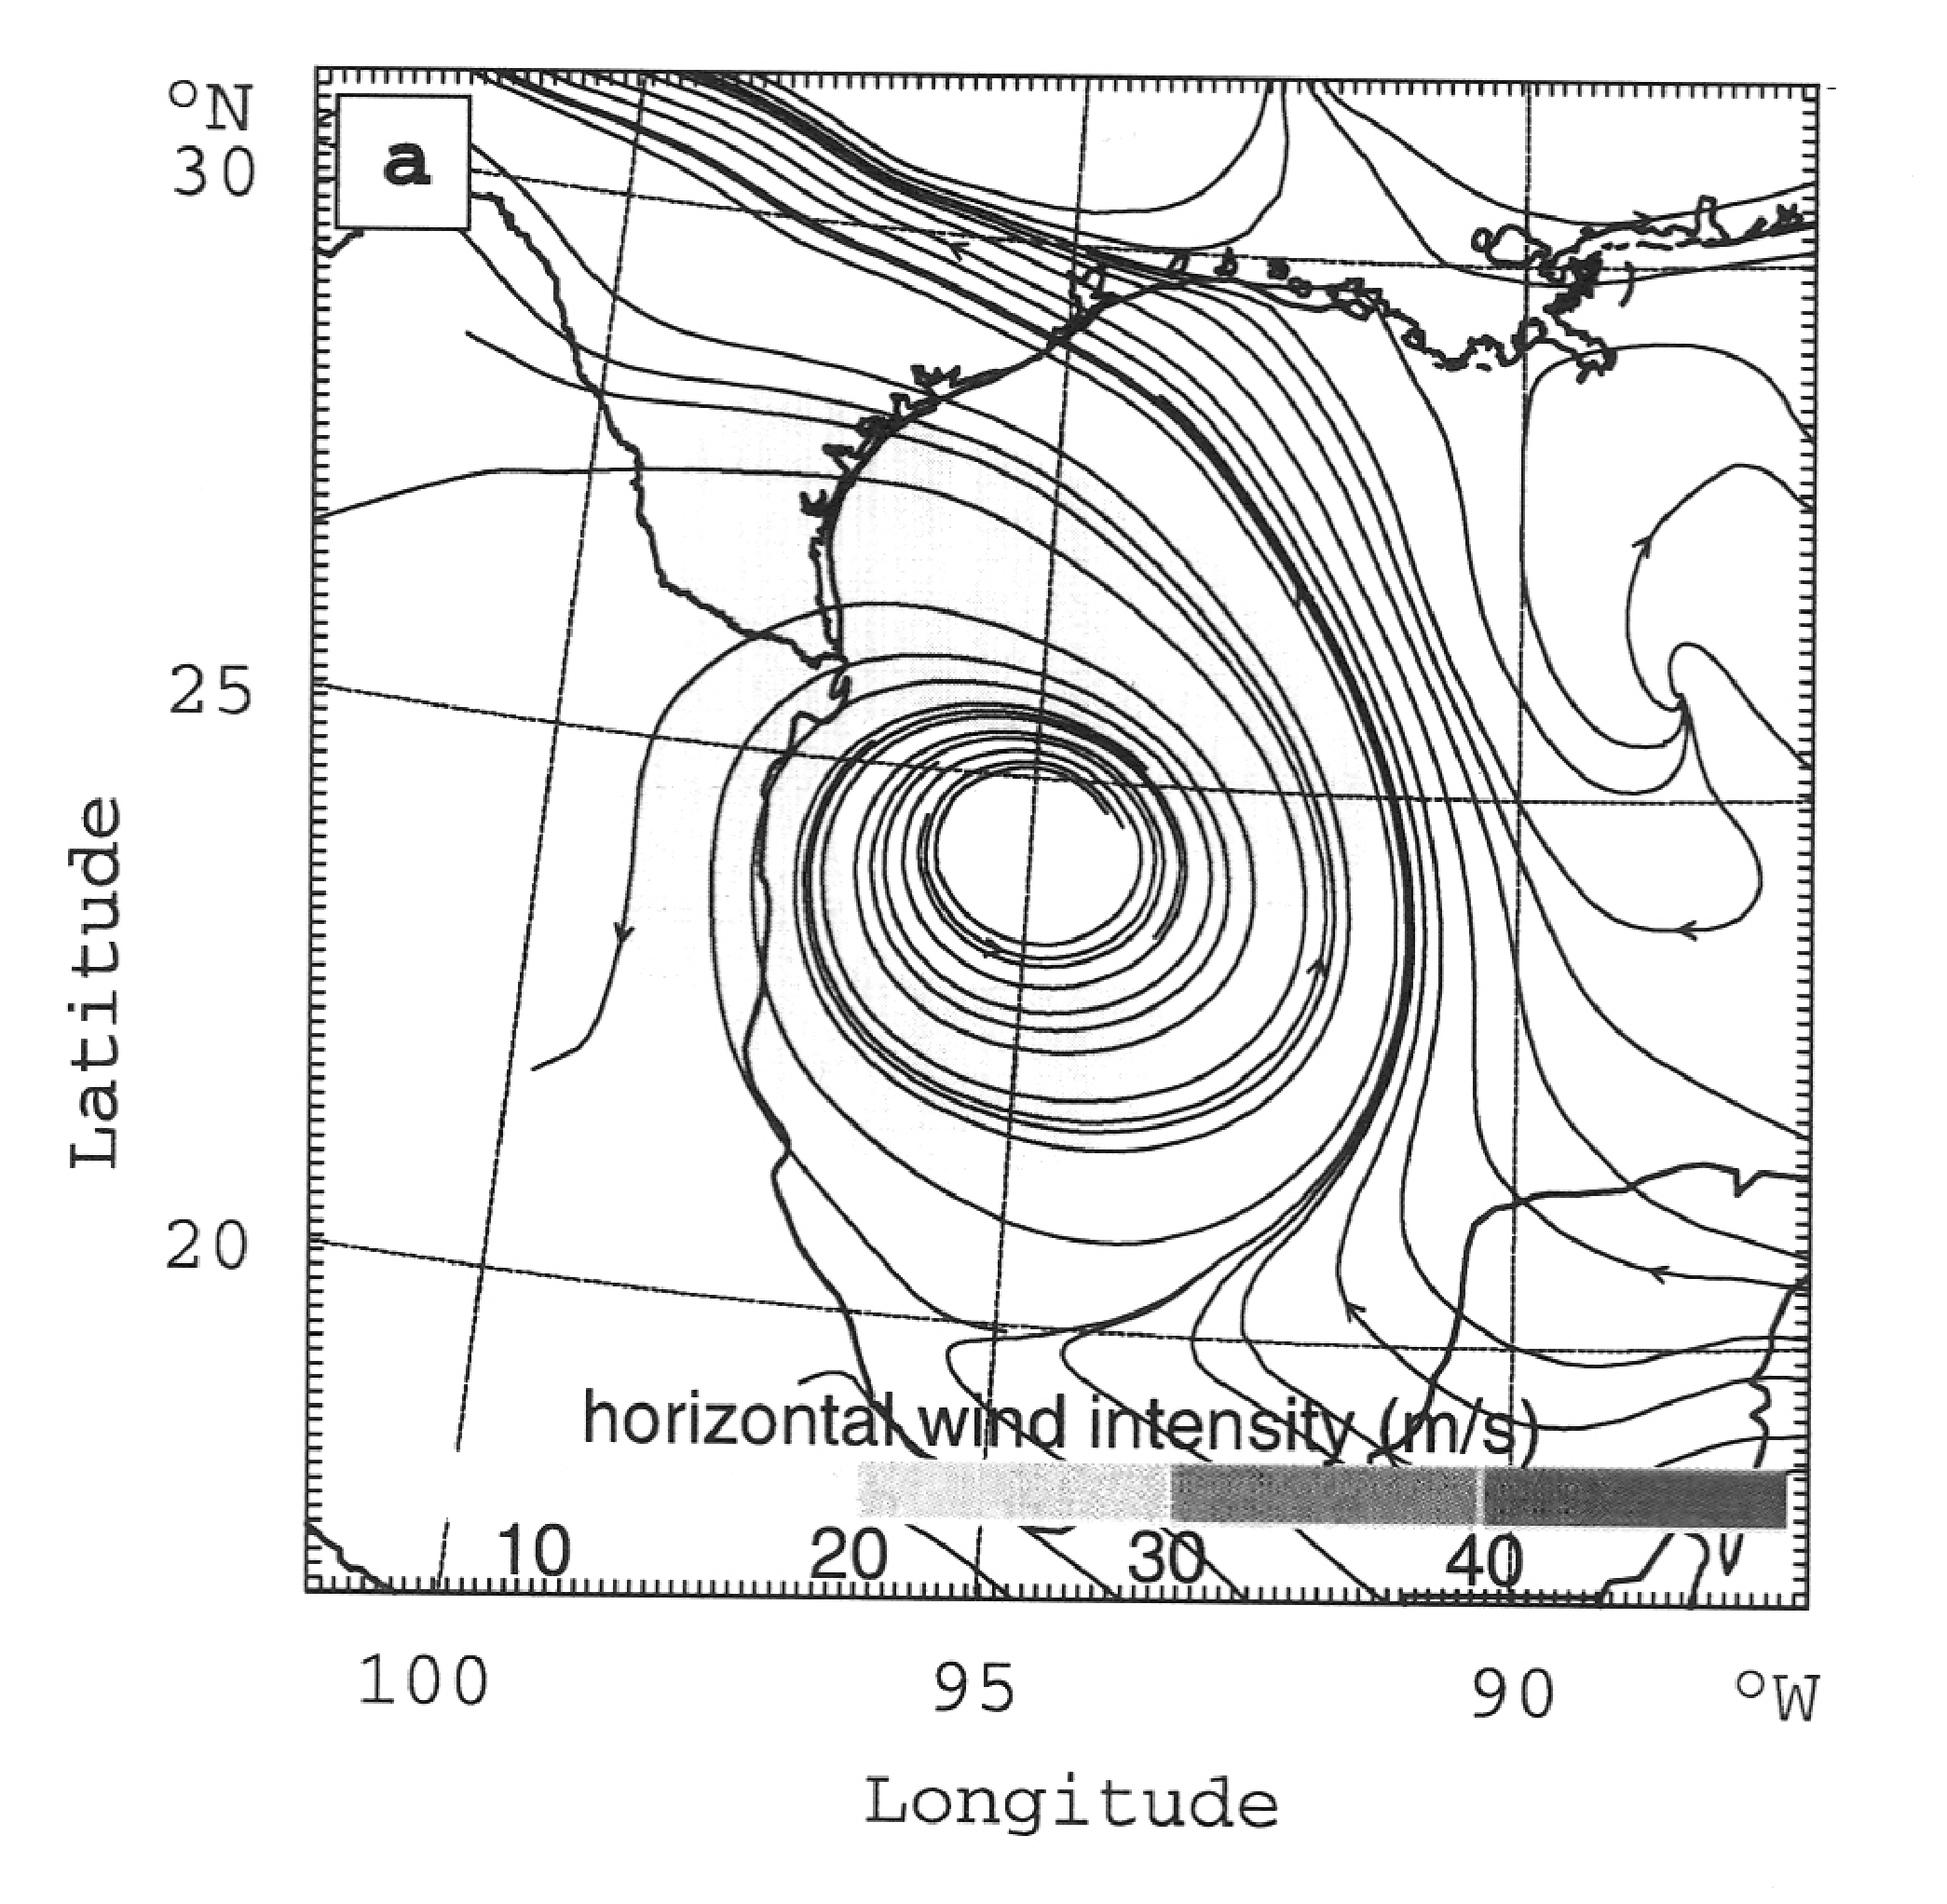
\includegraphics[width=8cm]{\EPSDIR/vortex_ecmwf.eps}&
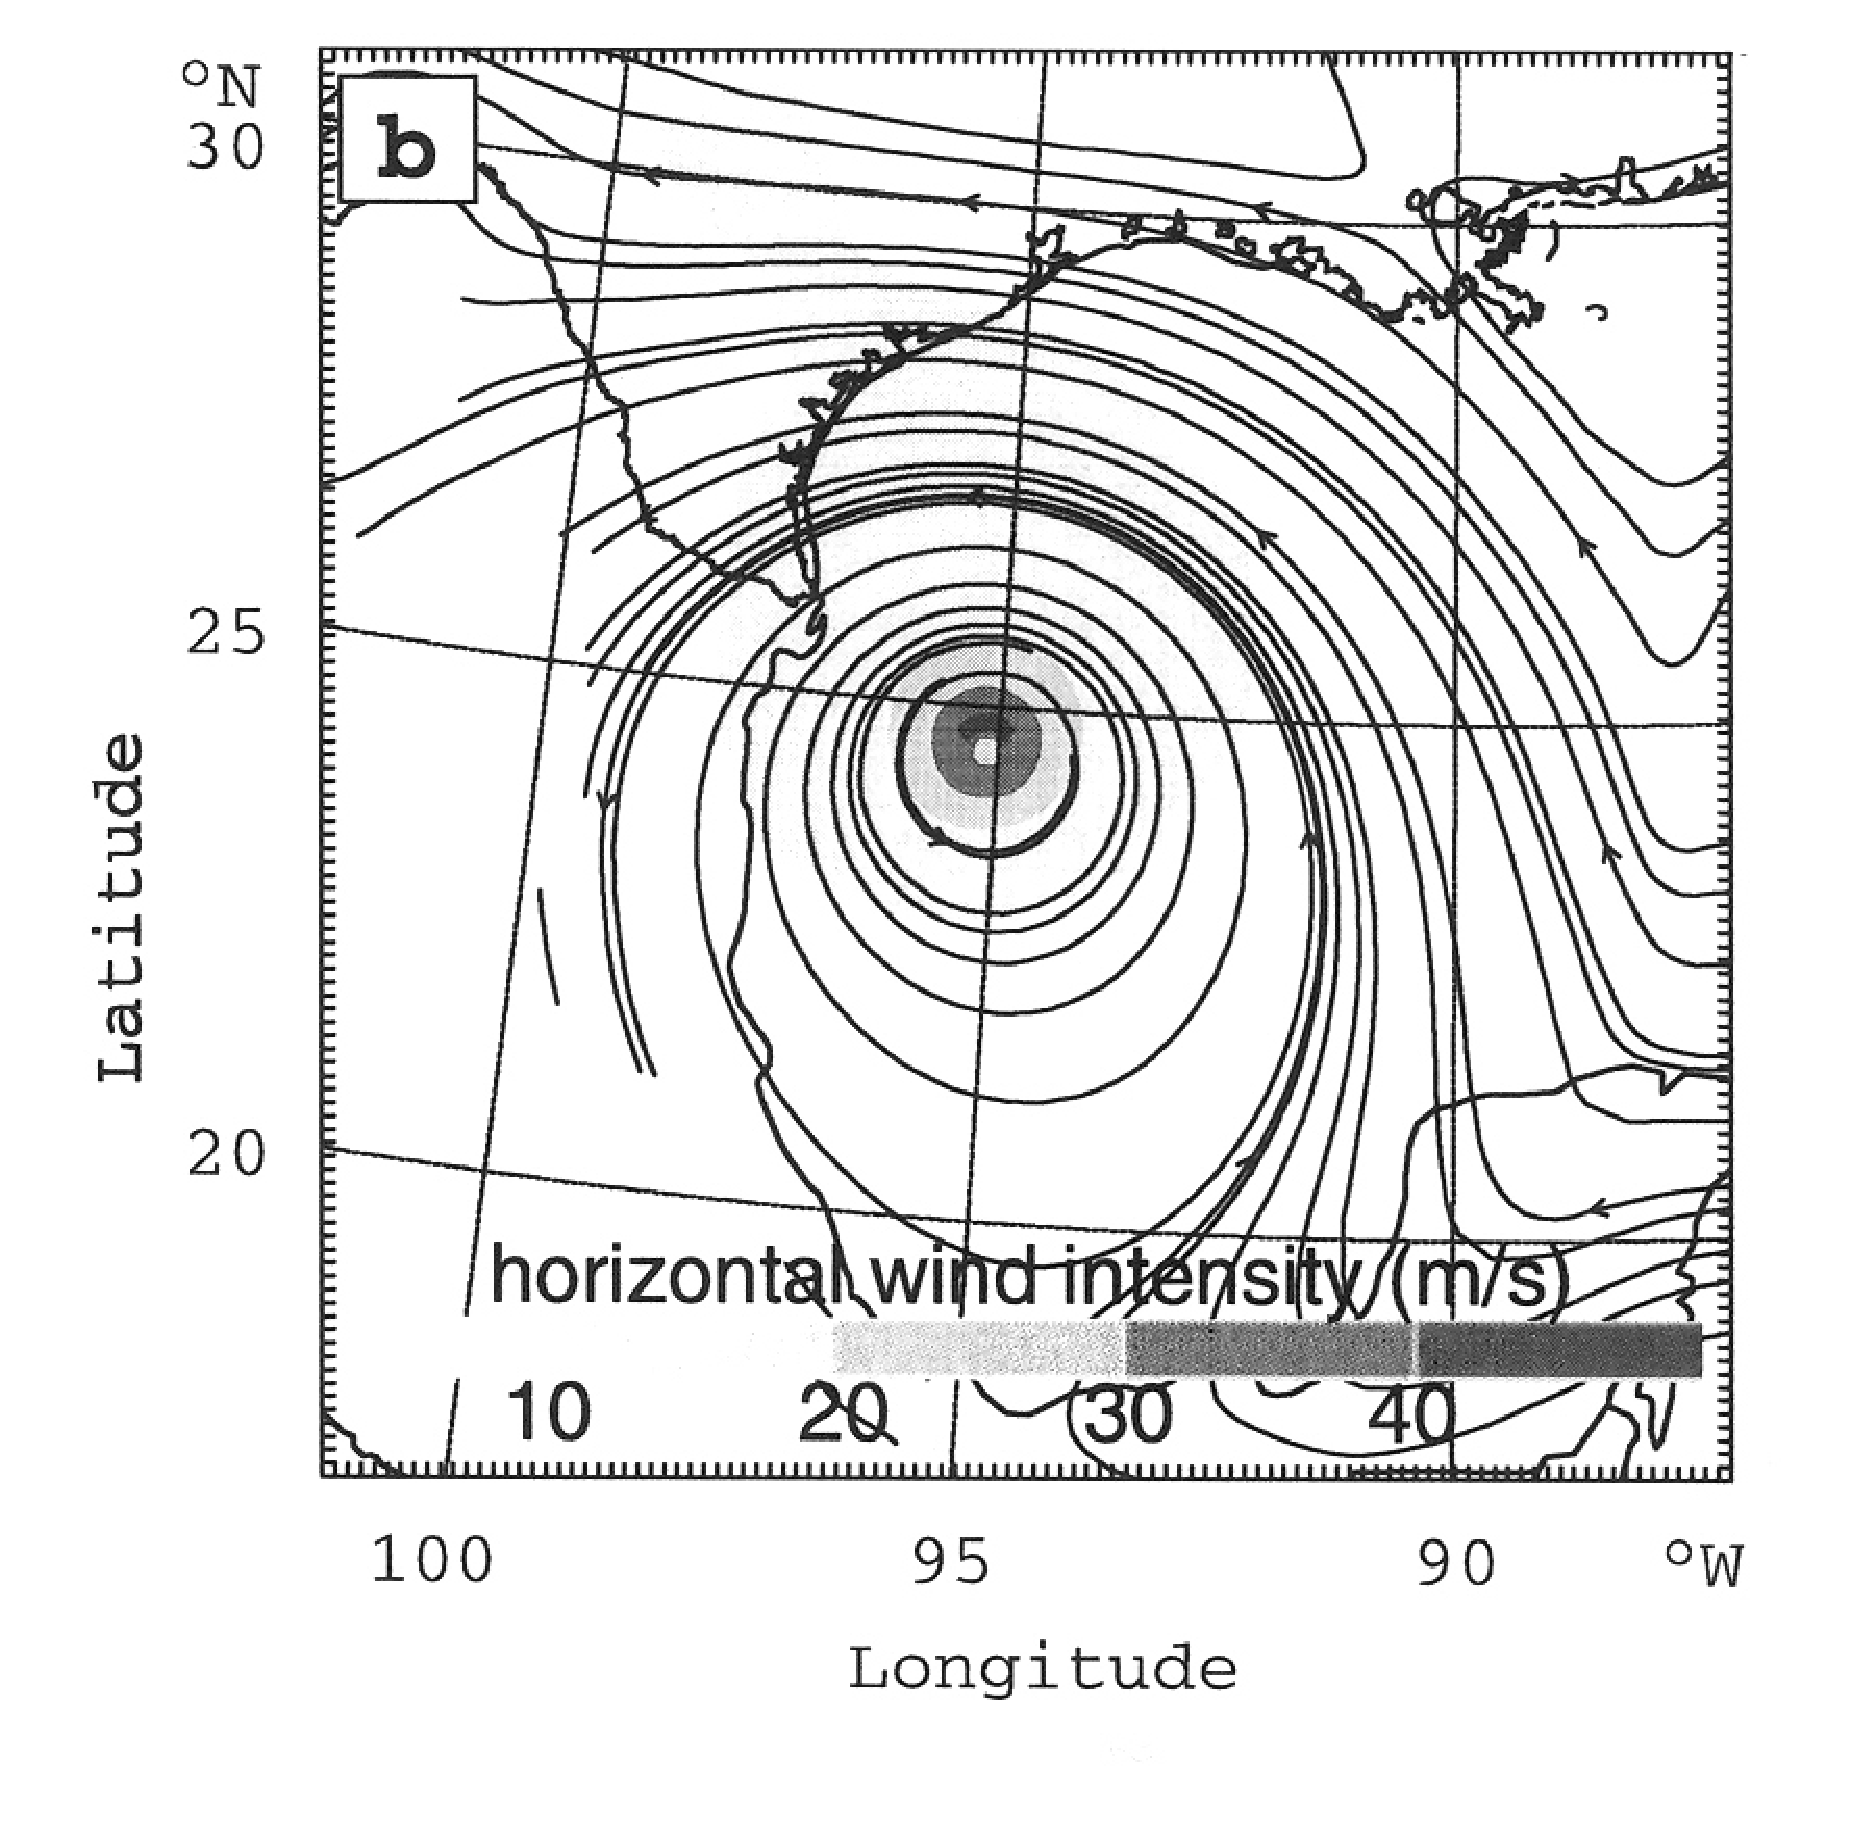
\includegraphics[width=8cm]{\EPSDIR/vortex_radar.eps}\\
\end{tabular}}
\caption{Horizontal streamlines at 850 hPa for Hurricane Bret on 22 August 1999 from (a) the ECMWF global analysis at 00 UTC and (b) the inclusion of the airborne Doppler-derived "specified"}
\label{bogus}
\end{figure}

\subsection{The radial circulation}

It must be emphasized that the EVTD analysis could permit to retrieve a realistic structure of the secondary circulation (i.e. updraft centered on the radius of maximum wind, inflow (outflow) in the lower (upper) part of troposphere). In  
numerical models (as in reality) the radial and vertical circulation results from: 
sensible- and latent-heat fluxes from the ocean surface increasing $\theta_{e}$ in 
the lowest atmospheric layers; surface friction inducing radial convergence; 
latent-heat release sustaining vertical motions through thermal buoyancy; and 
vertical momentum fluxes generating horizontal and vertical pressure perturbation 
gradients. Including these physical constraints in an analytical formulation of a 
symmetric secondary circulation would be a very difficult task.\\
However it is easy to include the effect of surface friction. Indeed according to the Ekman theory, the friction forces due to the surface (ocean or land) induce a radial convergence in the lower layers. The frictional verring (in radian) is given by:
\begin{equation}
\left \lbrace
\begin{array}{c c l c}
\label{eq_ekman}
\alpha^{Ekman}_{friction}(lat,z) &=& | z-H_{cl} |\times \sqrt{ \frac {|f|}{2K}} & \mbox{for} \ z<H_{cl}\\
&=& 0 & \mbox{for} \ z \geq H_{cl}\\
\end{array}
\right .
\end{equation}
where $H_{cl}$ is the height of the boundary layer and $K$ the Ekman exchange ratio (which is constant). It is therefore a linear function of altitude but independent of the wind and hence the distance from the centre. By cons, it is a function of latitude through the Coriolis parameter. However this theory leads to severe restrictions on the atmosphere that are not verified.
Climatological studies (Gray 1968, 1972) on tropical depressions can highlight a profile of inflow in low levels by friction. Such a climatological profile is characterized by (\ref{profil_conv_clim}), whatever the latitude and intensity of the wind (hence the distance from the centre of the system):
\begin{equation}
\left \lbrace
\begin{array}{c c l l}
\label{profil_conv_clim}
\alpha^{Clim}_{friction}(z) &=& 12^{\circ} & \mbox{for} \ 0 \leq z \leq 1000\,\mbox{m}\\
&=& 3^{\circ} & \mbox{for} \ 1000\,\mbox{m} <z \leq 2000\,\mbox{m}\\
&=& 0^{\circ} & \mbox{for} \ 2000\,\mbox{m} <z \\
\end{array}
\right .
\end{equation}
To include this convergence, the radial wind is calculated following the relation $V_{R}(r,z)=V_{T}(r,z) \times \tan \alpha_{friction}(z)$ where $V_{T}(r,z)$ is obtained by (\ref{VT(r,z)}) and $r \geq RMW$. We can notice that radial wind is nil for $r<RMW$, positive for an inflow and is no axisymmetric field because of the Coriolis parameter in $V_{T}(r,z)$. The user can choose the values of the friction angle but thought the climatological values are preferable, the default value being nil. For every point (i, j, k), the bogusing wind is:
\begin{equation}
\left \lbrace
\begin{array}{c c c}
U_{bog} &=& - V_{T} \sin \phi - V_{R} \cos \phi\\
V_{bog} &=& V_{T} \cos \phi - V_{R} \sin \phi\\
\end{array}
\right .
\end{equation}
where, for a vertical model level k, $\phi$ is the projection angle on the meridian axis of the vector $\overrightarrow{I_{bog}M}$, defined by the bogus center $I_{bog}$ and the considered point $M_{(i,j)}$.

\section{References}
\noindent
\por
Barnes, S. L., 1964:
A technique for maximizing details in numerical weather map analysis. {\it J. Appl. Meteor.}, {\bf 3}, 396-409.
\por
Gray, W. M., 1968:
Global view of the origin of tropical disturbances and storms. {\it Mon. Weather Rev.}, {\bf 96}, 669-700.
\por
Gray, W. M., 1972:
Diagnostic study of the planetary boundary layer over the oceans. {\it Technical Report 179}, Colorado State University.
\por
Holland, G. J., 1980:
An analytic model of the wind and pressure profile in hurricanes.
{\it Mon. Weather Rev.}, {\bf 108}, 1212-1218.
\por 
Kurihara, Y., M. A. Bender, and R. J. Ross, 1993:
An initialization scheme of hurricane models by vortex specification.
{\it Mon. Weather Rev.}, {\bf 121}, 2030-2045.
\por
Kurihara, Y., M. A. Bender, R. E. Tuleya, and R. J. Ross, 1995:
Improvements in the GFDL hurricane prediction system.
{\it Mon. Weather Rev.}, {\bf 123}, 2791-2801.
\por 
Nuissier, O., R. F. Rogers, and F. Roux, 2005:
A numerical simulation of Hurricane Bret on 22-23 August 1999
initialized with airborne Doppler radar and dropsonde data.
{\it Quart. J. Roy. Meteor. Soc.}, {\bf 131}, 155-194.
\por
Roux, F. and F. D. Marks Jr, 1996:
Extended Velocity Track Display (EVTD): An improved processing method for 
Doppler radar observations of tropical cyclones.
{\it J. Atmos. Oceanic. Technol.}, {\bf 13}, 875-899.
\por
Roux, F., F. Chane-Ming, A. Lasserre-Bigorry, and O. Nuissier, 2004:
Structure and evolution of intense tropical cyclone Dina near la R\'eunion on 22 
January 2002: GB-EVTD analysis of single Doppler radar observations.
{\it J. Atmos. Oceanic. Technol.}, {\bf 21}, 1501-1518.


